\subsubsection*{Planare Rekonstruction}

Der erste Proof of Concept Prototyp wurde zu Beginn dieser Arbeit auf Java Ebene implementiert und entwickelte sich nach und nach zu dem in \ref{sec:plane-reconstruction} beschriebenen Verfahren. Für die finale Umsetzung in dem nativen Prototypen mussten somit alle Algorithmen und Datenstrukturen neu in C/C++ umgesetzt werden. Begonnen wurde mit dem Octree, der in seinen tiefsten Zweigen die Menge aller aufgenommenen Punkte für den jeweiligen Sektor und eine Instanz der \enquote{Reconstructor} Klasse beinhaltet. Diese beinhaltet alle beschriebenen Algorithmen zur Ebenen Rekonstruktion wie RANSAC, die linearen Regression und den Graham Scan. 

\begin{figure}[h]
  \centering
	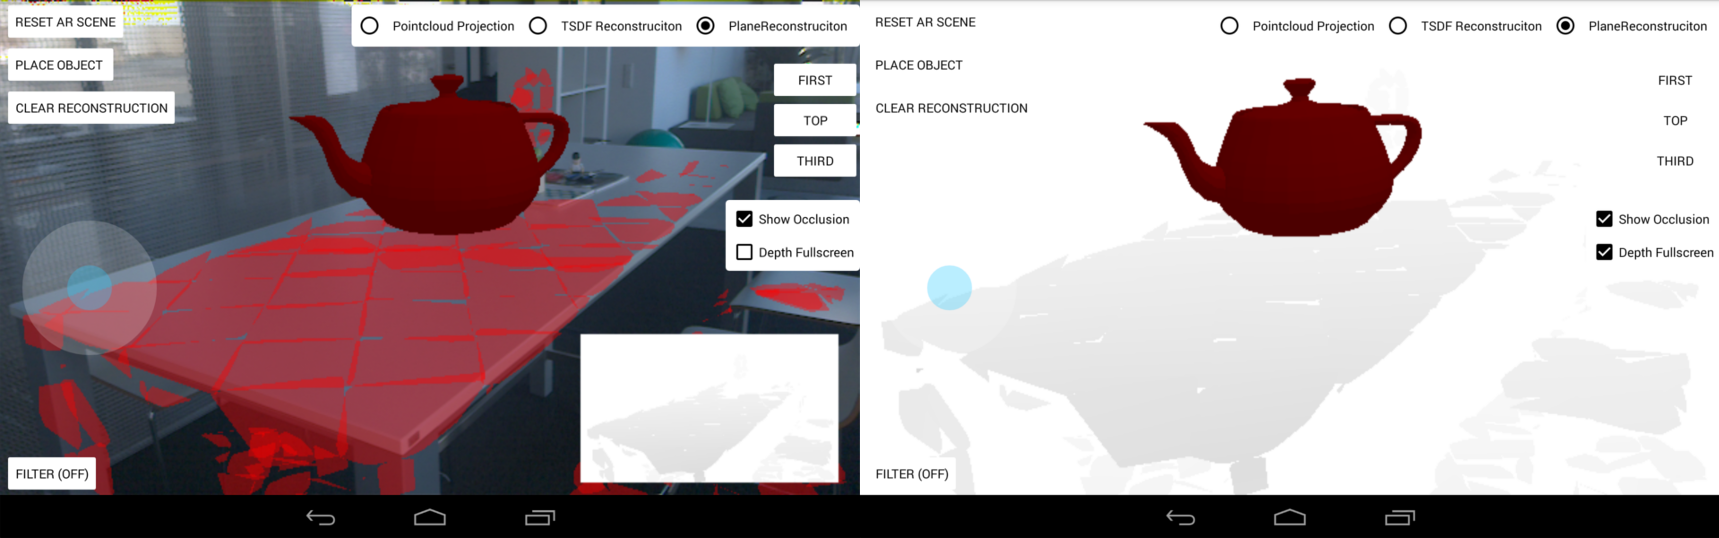
\includegraphics[width=1.0\textwidth]{content/images/implementation/plane-demo.png} 
  \caption{Planare Rekonstruktion Prototyp. Links optionale Projektion auf der Bildebene. Rechts das resultierende Tiefenbild.}
  \label{fig:plane-demo}
\end{figure}

Für die Berechnung mit Vektoren und Matrizen wurde wie auch im gesamten Projekt die OpenGL Mathematics Bibliothek (GLM)\footnote{OpenGL Mathematics - http://goo.gl/2oY83s (27.02.16)} verwendet. Sie bietet typische Primitiven mit entsprechenden Operationen für Berechnungen der linearen Algebra. Wie bereits beschrieben wird für die lineare Regression die Berechnung von Eigenvektoren mit ihren Eigenwerten benötigt. Diese Berechnung wird von GLM nicht unterstützt. Hier wurde die Eigen-Bibliothek\footnote{Eigen: template library for linear algebra - http://goo.gl/TsNOuW (27.02.16)} verwendet, die diese Operation für den Anwender anbietet. Abbildung \ref{fig:plane-demo} zeigt die Ergebnisse der Ebene Rekonstruktion Links und der daraus Resultierenden Tiefeninformation Rechts.


